% BEÁLLÍTÁSOK - JOBB NEM VÁLTOZTATNI
\documentclass[final]{ubb_dolgozat}

\usepackage{definitions}
\usepackage{caption}
\usepackage{enumitem}
\usepackage{multirow}
\usepackage[all]{nowidow}
\usepackage{hyperref}

\sloppy
\frenchspacing

\renewcommand{\baselinestretch}{1.5}
\setlength{\columnsep}{1cm}
\newenvironment{Figure}
{\par\medskip\noindent\minipage{\linewidth}}
{\endminipage\par\medskip}

% milyen nyelveken akarunk forráskódot megjeleníteni
%\lstloadlanguages{Java}

% ezt be lehet tenni MINDEGYIK megjelenítendő kód elé.
%\lstset{language=Java}

%% MELYIK ÉVBEN ADJUK LE
\submityear{%
2017
}
%% MELYIK HÓNAPBAN ADJUK LE
\submitmonthHU{%
Július
}
\submitmonthRO{%
Iulie
}
\submitmonthEN{%
July
}

\titleHU{%
Evolúciós játékok alkalmazása daganatos sejtek modellezésében
}

% Amennyiben szükséges, az alábbi sorokat ki kell komment-ezni és 
% beírni a megfelelő címeket

\titleEN{%
???Evolutionary games used to model cancerous cells
}

\titleRO{%
?
}

\author{%
Kis Nándor
}

%%
\tutorHU{%
dr. Gaskó Noémi,\newline egyetemi adjunktus\\
{\large Babe\c{s}--Bolyai Tudományegyetem,\\
 Matematika és Informatika Kar}% ha különbözik, akkor fel kell tűntetni
}
%%
\tutorRO{%
Adjunct dr. Gaskó Noémi\\
 {\large Universitatea Babe\c{s}--Bolyai,\\ % dacã diferã!!!
 Facultatea de Matematic\u{a} \c{s}i Informatic\u{a} }%
}
%%
\tutorEN{%
Adjunct prof. dr. Gaskó Noémi
 {\large Babe\c{s}--Bolyai University,\\
 Faculty of Mathematics and Informatics}
}

\begin{document}

%% ABSTRAKT
\begin{abstractEN} % ANGOL VÁLTOZAT

% a lenti részt értelemszerűen ki kell tölteni a dolgozat angol kivonatával.
% A BEGIN ... END között CSAK A SAJÁT SZÖVEG kell, hogy legyen.
% Az utolsó mondatot benne kell hagyni, mely által kijelentitek, hogy a munkátok SAJÁT.


{	???ANGOLUUUULLLL!!!
	Dolgozatunkban az evolúciós játékok alkalmazását mutatjuk be a sejtbiológiában. Már a sejtek szintjén megfigyelhetőek kooperatív illetve kompetitív viszonyok, amelyek játékelmélettel modellezhetőek. Ezeket, az alkalmazásunk elméleti háttereként is szolgáló matematikai modelleket használják a rákkutatásban is, ahol a sejtek mint játékosok vannak jelen. Fő célunk játékelméleti modellek kiterjesztése a sejtek interakcióinak vizsgálatára. A projekt gyakorlati részét egy webes felület képezi, amin megjeleníthető a különböző sejtpopulációk viselkedése, időbeni alakulása. A szimuláció paramétereit, a generációk számát a felhasználó módosíthatja, ezáltal valós időben betekintést nyerve a daganatok dinamikájába.
}

This work is the result of my own activity. I have neither given nor received unauthorized assistance on this work.

\end{abstractEN}

% ez a címoldal része
\maketitle

%% 

% a dolgozat tartalomjegyzéke -- ez automatikusan generálódik a STRUKTÚRA alapján.
{ \baselineskip 1ex
  \parskip 1ex
  \tableofcontents
}

\chapter{Bevezető}

A rákkutatás a mai napig egy nagyon aktív kutatási terület, melyben bizonyos matematikai modelleket is jól lehet alkalmazni. Ilyen például az evolúciós játékelmélet is, aminek a biológiai alkalmazása még egészen újnak számít. Dolgozatunk alapjait ezen területen írt legfrissebb munkák szolgálják. Az evolúciós játékelmélet segítségével a következőkben daganatos sejteket fogunk  modellezni és azok viselkedését kielemezni.

Dolgozatunkat több nagyobb részre osztjuk. Elsősorban szükségünk lesz néhány játékelméleti fogalomra, melyek nélkül a dolgozatot nem tekinthetnénk teljesnek. Itt kerülnek majd bevezetésre a játékok, ezek típusai és megismerkedünk az evolúciós játékelmélet alapjaival. Itt megemlítjük a fajon belüli rivalizálást és egy egyszerű példát az evolúciós játékra.

A következő fejezetben röviden részletezzük a daganatos sejteket és azok viselkedését, valamint az itt alkalmazható játékelméleti modelleket. Bemutatjuk az általunk használt modelleket, szereplőit és játékszabályait, valamint azt, hogy milyen újításokat tettünk hozzá az eredetihez képest. Azt is tárgyaljuk, hogy mik azok a Voronoi diagramok és miért pont azt használjuk.

Mindezt a sok elméleti fogalmat egy alkalmazásba csomagoltuk, így a következő fejezet bemutatja az alkalmazásunkat, amit egy webes felület képez, amelyen a fenti modellek jeleníthetőek meg, a sejtek viselkedése, a populáció időbeli alakulása és ezek statisztikája. Részletezzük az alkalmazás funkcionalitásait és felépítését, valamint a felhasznált technológiákról is beszámolunk.

Végül pedig összegezzük a szimulációk eredményét. Megvizsgáljuk, hogy az alkalmazás képes-e reprodukálni az eredeti modellt. Megnézzük, hogy a paraméterek változása hogyan befolyásolja a játék végkimenetelét és összevetjük az eredeti modellt a saját kibővített változatunkkal.

Itt megemlítenénk azt is, hogy ezen dolgozat egy kezdetlegesebb formája már bemutatásra került a XX. Reál- és Humántudományi Erdélyi Tudományos Diákköri Konferencián, ahol második díjjal lett jutalmazva.
\chapter{Evolúciós játékok}

\section{Klasszikus játékelméleti fogalmak}

A játékelméletet a matematika egy fő ágának tekintjük, mely olyan helyzetekkel foglalkozik, amelyben legalább két döntéshozó verseny helyzetbe kerül és saját nyereség függvényét próbálja maximalizálni. A nehézség abban rejlik, hogy minden szereplő befolyásolja legalább egy másik szereplő döntését. Ezen \textit{játékok} első elgondolásra társasági játékokra utalnak, de ezen játékokkal modellezhetünk közgazdaságtanban vagy szociológiában, katonai és biológia alkalmazásuk is létezik.

Bizonyos szempontok alapján, ezeket a játékokat, kategorizálni lehet. Itt kiemelhetjük a kooperatív játékot, amelyben a játékosok felismerve azt, hogy hasznot húzhatnak az együttműködésből, valamilyen szinten csoportosulnak. Illetve ennek párját, a nem kooperatív játékot, ahol a döntéshozó játékosok egymásnak versenytársai, bármiféle együttműködés önkéntes módon jöhet létre.

Egy másik osztályozási szempont szerint léteznek szimmetrikus játékok, ahol a haszon csak a választott stratégiától függ, a játékos személyétől nem. Aszimmetrikus játékról akkor beszélünk, ha a játékosok nem cserélhetőek fel anélkül, hogy a stratégiák nyereségén változtatnánk.

\subsection{Statikus és szekvenciális játékok}
Minden játék esetén szükségünk van az idő fogalmára, így eszerint két típusúról beszélhetünk. A statikus játékok esetében a döntéshozók már a játék legelején, egymástól függetlenül döntenek. Ezzel szemben, a dinamikus játékok esetében számít a lépések sorrendje, mivel minden döntéshozó ismeri az a többiek előző lépéseit. Amennyiben egy statikus játékot ismételten játszanak, úgy azt a dinamikus kategóriába sorolhatjuk, hiszen egy kör elején az eddigi körök alapján hozza meg döntését egy játékos. Ezen két típusú játék ábrázolása is különbözik egymástól. A statikusokat általában egy mátrix segítségével írjuk le, amelyről leolvasható az összes lehetséges kimenet. Míg a dinamikusok esetében egy véges irányított fa ábrázolja az egymás utáni lépéseket, amely gyökere a kezdőállapot, ahonnan bármely ponthoz egyetlen egy út vezet.

\subsection{Nash-egyensúly}
Amennyiben a játék során létrejön egy olyan állapot, ahol egyik döntéshozónak sem éri meg eltérni a saját alkalmazott stratégiájától, egyik fél sem akar változtatni, akkor az úgynevezett Nash-egyensúlyról beszélünk. Tekintsük \(G = ((N,S_i,u_i), i = 1,...,n)\) rendszert egy véges stratégia játék reprezentációjának, ahol \textit{N} a játékosok halmaza, \textit{n} pedig a játékosok száma. Minden \(i \in N\) játékos a \(S_i\) lépés-halmazból választhat. \(S = S_1 \times S_2 \times ... \times S_n\)  a játék összes kimenetelének halmaza, ahol \(s \in S\) egy stratégia-együttes. Minden \(i \in N\) játékos nyereségét a \(u_i:S \to \mathbb{R}\) hasznosságfüggvény írja le. Jelöljük \((s_i^*,s_i) = (s^*_1,...,s_i,...,s_n^*)\) -vel azt a stratégia-együttest, amelyet az \(s^*\)-ból kapunk ha az \textit{i} játékos stratégiáját kicseréljük \(s_i\)-re. Egy \(s^*\) stratégia-együttes Nash-e\-gyen\-súly\-ban van, ha az \(u_i(s_i^*,s_i)\leq u_i(s^*) \) egyenlőtlenség igaz \(\forall i = 1,...,n, \forall s_i \in S_i, s_i \ne s_i^*\) esetén \cite{nash1951non}.


\section{Játékelmélet a biológiában}
Az evolúciós játékelmélet a játékelmélet biológiai alkalmazása során jött létre, a fejlődő populációk vizsgálata a biológiában. Maynard Smith volt az aki felismerte, hogy a játékosoknak nem feltétlenül kell racionálisan viselkedniük, már az is elegendő ha van egy stratégiájuk. A stratégiák genetikailag öröklődnek, ezek befolyásolják egy egyed jellegét. Attól függően, hogy egy stratégia milyen gyakori illetve milyen más stratégiák vannak még jelen a játékban, meghatározható egy adott stratégia sikeressége. A résztvevők szelekciós sikerét a \textit{fitnesz} fejezi ki (a szaporodásra való relatív esély). Egy stratégiát evolúciósan stabilnak nevezünk, ha az azt alkalmazó populáció nem győzhető le semmilyen más, kezdetben kevés létszámú stratégiával. Az evolúciós játékelméletben az egyensúlyt az evolúciósan stabil stratégia jelenti.

Például egy egyszerű evolúciós játék a következő. Tegyük fel, hogy adott egy bogár populáció, amely ételért verseng (\cite{book:egt}). Az egyszerűség kedvéért csak két stratégia lesz, a bogarak vagy kicsi- vagy nagytestűek. Nem meglepő, hogy a nagyobb testű bogarak több ételhez jutnak hozzá ha kisebb társaikkal versenyeznek. Ha két bogár egymással versenyez, akkor a következő kimenetelek lehetségesek:
\begin{itemize}[noitemsep]
	\item ha két egyforma méretű bogár verseng, akkor egyformán osztják el az ételt
	\item ha egy kicsi és egy nagy verseng, akkor természetes, hogy a nagyobbiknak sokkal több jut
	\item mindkét esetben a nagytestűek az étel egy részét elveszítek, ezt a versengés emészti fel 
\end{itemize}
A játékot legkönnyebben egy payoff mátrixszal lehet leírni ahogyan azt a \ref{fig:beetle} táblázat teszi. Jól látható, hogy a táblázatban szereplő értékek megfelelnek a fenti szabályoknak. Az is látható, hogy ha két nagy bogár verseng, akkor mindkettejüknek sokba kerül a verseny.
Ekkor látható a legjobban, hogy míg a hagyományos játékelméletben a döntéshozók stratégiát választhatnak, addig itt egy egyed örökölte a stratégiáját. Egy nagytestű bogár nem dönthet úgy, hogy ő most kicsi testtel szeretne versengeni, erre nincs lehetősége. Itt a Nash-egyensúlynak már kevesebb értelme van, ezért az lecserélődik evolúciósan stabil stratégiára mint egyensúlyi állapot.

\begin{table}[htb!]
	\centering
	\begin{tabular}{ccccc}
		&       & \multicolumn{2}{c}{Bogár2} &  \\
		\multicolumn{1}{c}{}    &       & Kicsi        & Nagy        &  \\ \cline{3-4}
		\multirow{2}{*}{Bogár1} & Kicsi & \multicolumn{1}{|c|}{5,5}          & \multicolumn{1}{c|}{1,8}         &  \\ \cline{3-4}
		& Nagy  & \multicolumn{1}{|c|}{8,1}          & \multicolumn{1}{c|}{3,3}         & \\ \cline{3-4} \\
	\end{tabular}
	\caption{Bogár játék testméret alapján}
	\label{fig:beetle}
\end{table}
\chapter{Daganatos sejtek modellezése}
A tumorkeletkezés leggyakoribb oka az emberi génállományban található, a növekedést szabályozó gén aktiválódása. Ez vezet a szövetregeneráció során rendellenes utódsejtek képzéséhez, amelyek az egészséges szövetbe betörve versenyeznek az erőforrásokért. Többféle daganatos sejt is kialakulhat, mind különbözőképp hatva a környezetére, és így egy olyan változatosság alakulhat ki amely segíti az elszaporodást, egyre erősebben képes ellenállni a kezeléseknek. A játékelmélet egy lehetséges eszköz lehet az ezek közötti versengés modellezésére.

\begin{figure}[h!]
	\centering
	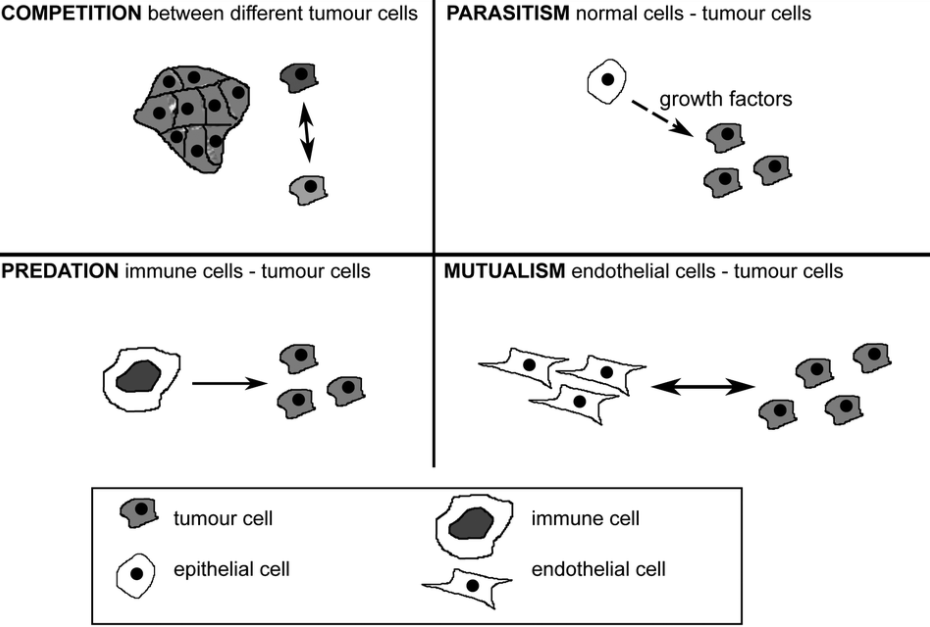
\includegraphics[width=90mm]{images/models}
	\vspace*{2mm}
	\caption{Daganatos sejtek közötti verseny típusok (\cite{hummert2014evolutionary})}
	\label{fig:cancerModels}
\end{figure}

A evolúciós játékelméleti modellek segítségével többféleképpen is megközelíthető a probléma. Játékosok lehetnek csak a daganatos sejtek és a játékot az erőforrásokért folytatott \textit{verseny} jelenti. Ez a verseny átalakulhat \textit{parazitizmussá} ha a bizonyos növekedési faktorokat termelő egészséges sejteket tekintjük az egyik félnek, és az ezt kihasználó daganatos sejteket a másiknak. Az immunsejtek játszhatják a \textit{ragadozó} szerepét de felléphet \textit{mutualizmus} is például az erek belső rétegének sejtjei és a daganatos sejtek között (\ref{fig:cancerModels}). 

\section{Közjó játék (Public goods game)}
A daganatos sejtek több jellegzetességének kialakulásában fontos szerepet játszanak az általuk termelt növekedési faktorok és jelzőmolekulák. Ezek segítenek többek között abban, hogy a rákos sejtek a saját növekedésüket ösztönözzék, hogy képesek legyenek kijátszani a szervezet védekezési rendszerét és hogy szétterjedjenek távoli szövetekbe (metasztázis). Mivel ezek az anyagok kikerülnek a sejtek közötti térbe, nem csak az őket termelő sejtekre vannak hatással, hanem az ezeket körülvevőkre is. Így a növekedési faktor felfogható mint egy "közös jó" (\textit{public good}). Az evolúciós játékelmélet megfelelő keretet biztosít, mivel nem feltételez racionális viselkedést és egy stratégia sikerességét megadja a populáción belüli gyakorisága \cite{archetti2016cooperation}.

\section{A játék felépítése}

A mai napig két modellt sikerült áttanulmányoznunk és az alkalmazásba beépítenünk. Ezek közül a \cite{archetti2016cooperation} cikkbeli modellt ezen dolgozatban fogjuk részletezni és a továbbiakban az alkalmazás csak azon részét mutatjuk be amely ezzel foglalkozik, míg a másik modell, amely a Warburg hatással is foglalkozik (\cite{archetti2014evolutionary}), a {\color{red} Réka ref} dolgozatban van ismertetve. 

\subsection{Voronoi diagram}
Az általunk vizsgált modell eltér a megszokottól abban, hogy a sejtek ábrázolására Voronoi hálózatokat használ. Térbeli játékok esetén általában szabályos pontrácsokkal vagy skála-független hálózatokkal dolgoznak. Míg az előbbi figyelmen kívül hagyja a kapcsolatok sokféleségét, az utóbbi nem megfelelő, ha az egyedek egy síkban helyezkednek el \cite{archetti2016cooperation}.

Legyen egy \textit{X} metrikus térben \textit{d} a távolságfüggvény, \textit{K} indexhalmaz, \(\{P_k\}_{k \in K}\) pedig \textit{X} nemüres résztereinek listája. A \(P_k\)-hoz tartozó \(R_k\) Voronoi cella a \(P_k\)-hoz legközelebbi pontok halmaza: 
\begin{equation}
R_k = \{x \in X | d(x,P_k) \leq d(x,P_j), \forall j \neq k\}
\end{equation}
ahol \(d(x,A) = inf\{d(x,a)|a \in A\}\) \textit{x} pont távolságát jelöli \textit{A} résztértől. Egy Voronoi diagram Voronoi cellák rendezett listája
  

\subsection{A játék szereplői és a stratégiák}
A játékban résztvevő sejtek két stratégia közül választhatnak: \textit{kooperálnak}, azaz termelnek növekedési faktorokat, vagy \textit{defektálnak}, azaz nem vesznek részt a faktorok termelésében. A stratégiák \textit{nyereségének (payoff)} kiszámítására a következő képletet használtuk: \(p = b(j) - c\) ahol a \textit{c} a növekedési faktor előállításának költsége, \textit{j} a csoportban résztvevő kooperatív sejtek száma és
\begin{equation}
b(j) = [V(j) - V(0)]/[V(n) - V(0)]
\end{equation}
a
\begin{equation} \label{eq:payoffGradient}
V(j) = 1/[1 + e^{(-s(j-k)/n)}]
\end{equation}
függvény normalizált alakja. A \textit{k} befolyásolja az áthajlási pont helyét, az \textit{s} irányítja a függvény meredekségét az áthajlási pontban. A vizsgált csoport méretét az \textit{n} jelöli. 

A kezdeti populációban véletlenszerűen elhelyezünk defektáló sejteket (alapértelmezetten az arányuk 0.05). Ezután minden körben véletlenszerűen kiválasztunk egy sejtet és annak egy szomszédját és megvizsgáljuk a nyereségeket. Amennyiben a szomszéd stratégiája kifizetődőbb, a kiválasztott sejt átveszi azt. Minden kör végén aktualizáljuk a nyereségeket, hiszen a stratégiák változtatásával változik a \textit{j} értéke és azzal a nyereségek is (aszinkron módon számolunk). 

\subsection{Diffúziós távolság}
A dolgozatunkban vizsgált modell másik újítása, hogy nem csak az elsőfokú szomszédokat veszi figyelembe, hanem egy bizonyos diffúziós távolságon belül található összes sejtet. A szomszédos termelő sejtek befolyásának súlyozására egy diffúziós gradienst vezetünk be. 
\begin{equation}
G(i) = [g(i) - g(0)]/[g(D) - g(0)] 
\end{equation}
és
\begin{equation} \label{eq:diffGradient}
g(i) = 1/[1 + e^{(-z(i-d)/D)}]
\end{equation}
függvények segítségével kiszámolhatjuk az \textit{i} távolságra található kooperatív sejtek befolyásának mértékét. Így a termelők száma nem a fent említett \textit{j} lesz, hanem a \textit{G}-vel kiszámított súlyozott összeg. A képletben szereplő \textit{d} és \textit{D} a diffúziós gradiens alakját határozzák meg, a \textit{z} a gradiens meredekségét az áthajlási pontban \cite{archetti2016cooperation}. Ezzel a modellünk jobban visszaadja azt ami a valóságban történik, hisz a sejtek nem csak a közvetlen szomszédokkal vannak kölcsönhatásban, hanem távolabbiakkal is.

\section{Osztódás}
Kezdeti szimulációink során nem vettük figyelembe azt, hogy a sejtek életük során szaporodni, azaz osztódni is szoktak, ezért mint saját újítás beépítettünk a modellbe egy osztódási lehetőséget is. 

A legtöbbet használt modell, mely elég közel áll a természethez, az a Gompertz modell \cite{wiki:gompertz}, amely leírja a tumor méretének időbeli változását a következő képlettel:
\begin{equation}
	\label{eq:gompertz}
	n_t = K \bigg(\frac{n_0}{K} \bigg) ^ {e^{(- \alpha t)}},
\end{equation}
ahol $n_t$ a populáció mérete a $t$ időpillanatban, $n_0$ a populáció kezdeti mérete, $K$ az elérhető maximális mérete a tumornak, míg az $\alpha$ egy konstans, mely a sejtek burjánzási képességével áll összefüggésben. Ez a modell nem csak egy valósághoz közeli képet ad, de azt is biztosítja, hogy a sejtek száma nem nő túl nagyra, mert az a szimulációs rész során komoly lassuláshoz vezetne. 

A játék során használt modellbe könnyen beépíthető, viszont nem veszi figyelembe azt, hogy éppen milyen típusú sejt (kooperáló/defektáló) osztódik. Ez nem azt jelenti, hogy az eredmény amit így kapunk nem elég pontos, hanem azt, hogy nem minden esetben jó ez a megközelítés. Az is megtörténhet, hogy a defektáló sejtek gyorsabban terjednek mint a kooperálók és így egy hibás képet kapunk a játékról.
\newcommand{\projectName}{Az EGTIB}

\chapter{\projectName{} bemutatása}

\projectName{} projekt célja egy olyan felhasználóbarát felület létrehozása, mely lehetőséget teremt a daganatos sejtek játékelméleti modellezésére és szimulációjára, a szimulációs eredmények megjelenítésére illetve ezeknek valamilyen szintű mentésére is. Ezért született meg, a mai trendeket figyelembe véve, egy kliens-szerver architektúrán alapuló webalkalmazás, mely részben az \cite{archetti2016cooperation}-ben megjelent modellt implementálja, és ahhoz új funkcionalitásokat is hozzáad.

\begin{figure}[ht!]
	\centering
	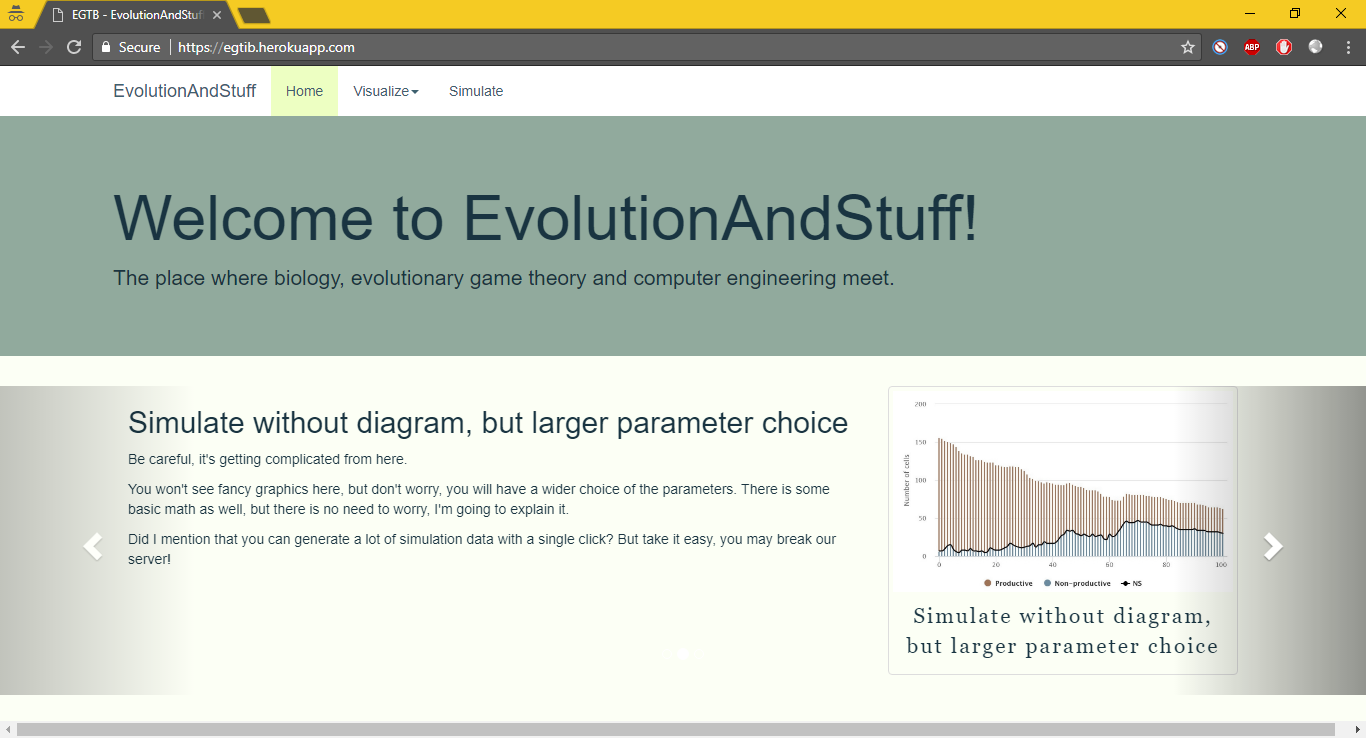
\includegraphics[width=0.98\linewidth]{images/welcomePage}
	\vspace*{1mm}
	\caption{Főoldal}
	\label{fig:welcomePage}
\end{figure}

\section{Funkcionalitások}

Az alkalmazásunkat egy főoldalra, valamint funkcionalitás szerint, három fő komponensre oszthatjuk:

\paragraph{Üdvözlő oldal}- ezen az oldalon kaptak helyet az általános jellegű információk és egy boostrap carousel, amellyel az alkalmazás mindegyik fő komponense rövid és humoros szövegekkel van bemutatva, valamint egy kép amely tovább visz az adott oldalra (Ábra \ref{fig:welcomePage})

\paragraph{Vizualizáció}- a vizualizációs oldalra tévedve (\ref{fig:VisualizationDiagram}), a felhasználó elég sok újdonsággal találja magát szemben. Az legszembeötlőbb egy színes pöttyökkel teli rajz lesz, ami a Voronoi diagram. Itt a kooperáló és defektáló sejtek narancssárga illetve sötétbarna színben vannak reprezentálva. A képernyő második legnagyobb részét a diagramtól balra elhelyezkedő paraméterlista tölti ki. Itt a következő paramétereket lehet állítgatni, amelyek a szimulációt befolyásolják:
\begin{itemize}
	\item kezdeti populáció mérete
	\item defektálók aránya 
	\item generáció szám (szimuláció hossza)
	\item kooperáló sejtek termelési költsége 
	\item diffúziós távolság mérete
	\item akarja-e a felhasználó, hogy a sejtek osztódásra legyenek képesek
\end{itemize}

\begin{figure}[ht!]
	\centering
	\captionsetup{justification=centering}
	\begin{tabular}{cc}
		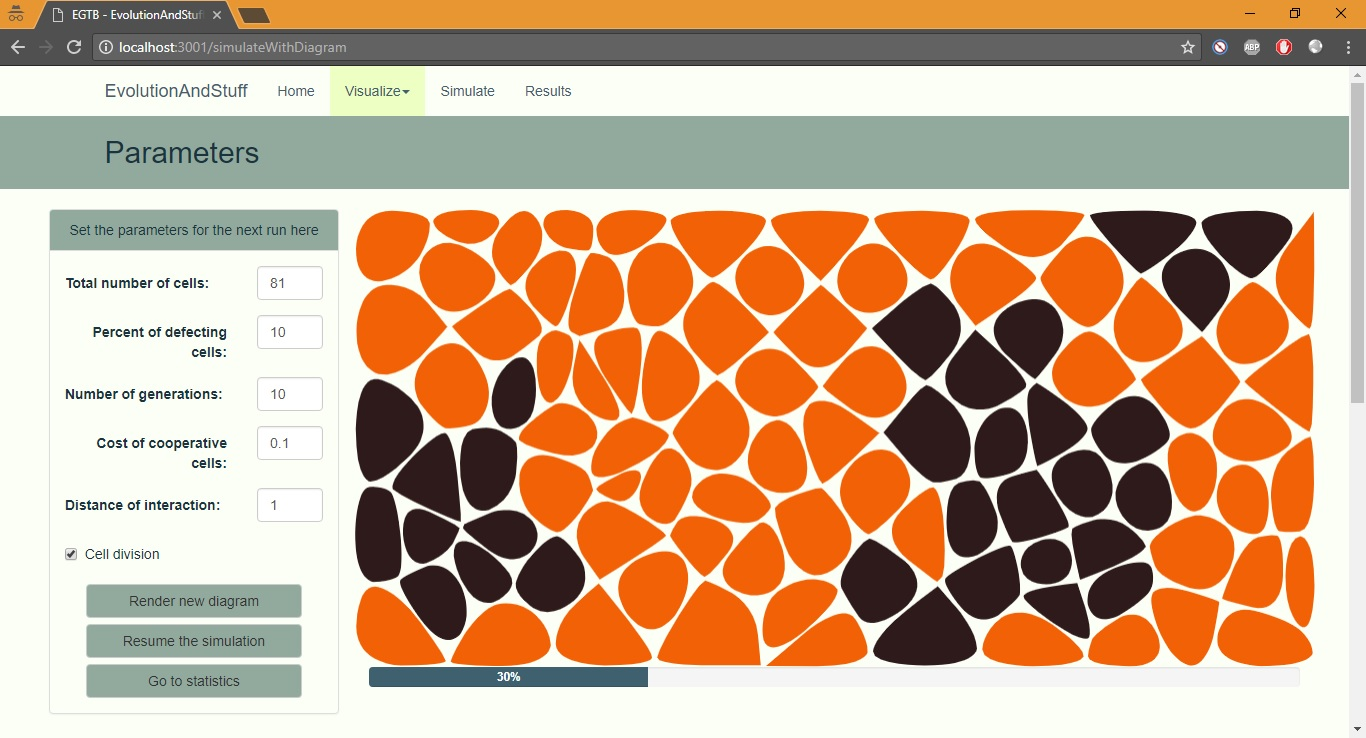
\includegraphics[width=0.47\linewidth]{images/EGTIB}
		&
		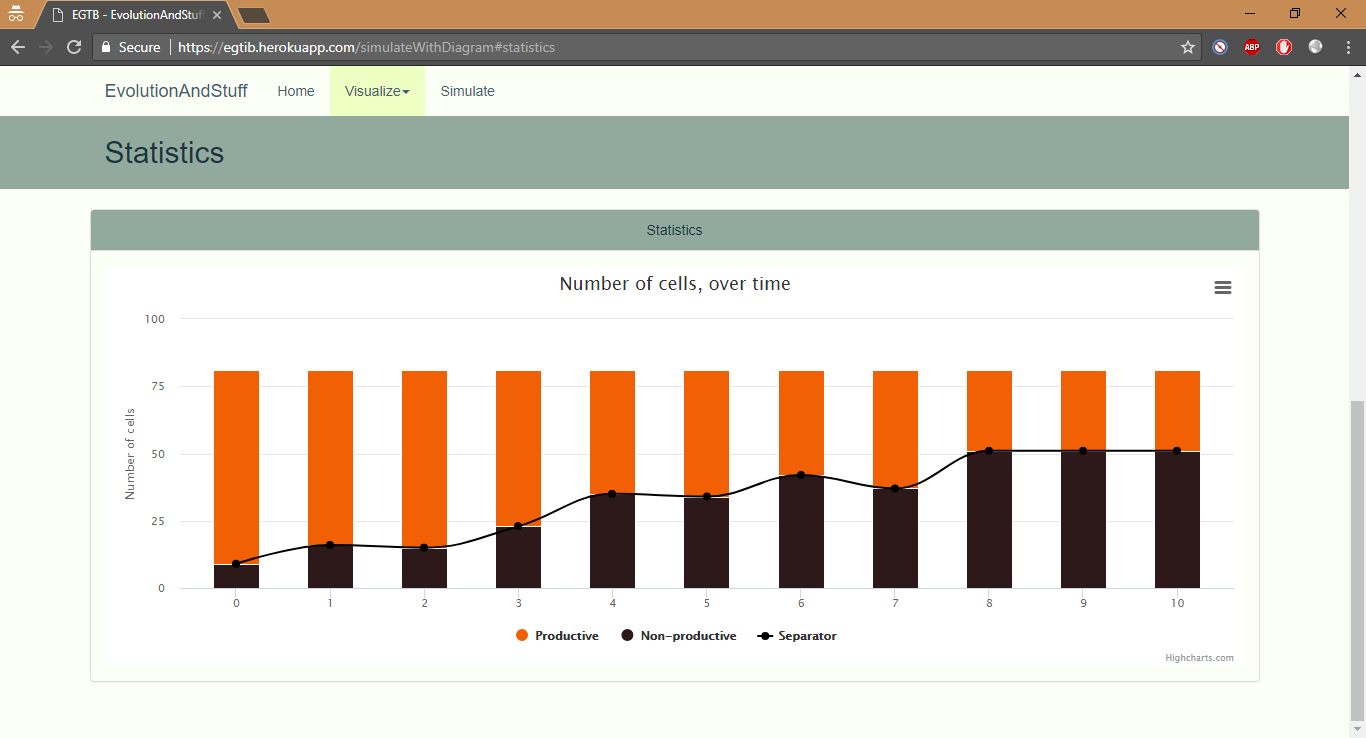
\includegraphics[width=0.47\linewidth]{images/VisualizationDiagram}
	\end{tabular}
	\caption{Bal: vizualizációs oldal, Voronoi diagram, paraméterek. Jobb: a populáció változása generációnként adott paraméterekre}	
	\label{fig:VisualizationDiagram}
\end{figure}

A paraméterlista alatt található az új Voronoi diagramot generáló gomb is. Erre szükség van, mivel minden paraméter változásnál a Voronoi diagramot újra kirajzolni túlságosan költséges lenne és nagyon belassítani az oldalt, ezzel rontva a felhasználói élményt. A szimuláció elindításáért felelős gomb is itt kapott helyet, amely a szimuláció során megállít és folytat gombra cserélődik, attól függően, hogy a szimulációt megállítjuk-e. Amennyiben a felhasználó lusta lenne letekerni az oldal aljára, elhelyeztünk számára egy statisztikához ugró gombot is. Ha a felhasználó egy kicsikét leleményes, akkor rájön arra is, hogy amennyiben megállítja a szimuláció lejátszását, a Voronoi diagram alatt elhelyezett progress bar segítségével tekergetheti a szimulációt, pont úgy mint egy filmet.
Megszorítása ezen oldalnak, hogy 500 sejtnél többet nem lehet vele kirajzoltatni, illetve szimulálni, mert annak kirajzolása túlságosan költséges, a felhasználó csak annyit érzékelne, hogy az oldal megfagyott.

\paragraph{Szimuláció}- erre az oldalra (\ref{fig:SimulationFunctionDiagrams} ábra) kerültek az átlag felhasználónak nem sokat mondó paraméterek, valamint a sejtek száma is csak annyira korlátozott, amennyit a szerver képes szimulálni (max. 2000 sejt). Első szembeötlő eltérés a vizualizációs oldalhoz képest az, hogy itt már nincs Voronoi diagram, többek között ezért sincs annyira megkötve a sejtek maximális száma. Itt már nem kerül kirajzolásra a szimuláció, de természetesen a statisztikás grafikon itt is megjelenik. A felhasználó belenyúlhat az alábbi paraméterekbe is ezen az oldalon:
\begin{itemize}
	\item a V függvény meredeksége
	\item a V függvény áthajlási pontjának helye
	\item a gradiens alakja
	\item a gradiens meredeksége az áthajlási pontban
\end{itemize}
Mivel ezek csak nyers számok, ezért jó ötletnek gondoltuk azt, hogy a  V (\ref{eq:payoffGradient} képlet) és g (\ref{eq:diffGradient} képlet) függvényeket jelenítsük meg. Ezen grafikonok elhelyezése egyszerű volt, hisz a Voronoi diagram helyét vették át. Itt a paraméterek változtatása interaktív, ami annyit jelent, hogy amint a paraméter értékét átírjuk, úgy a grafikon is annak megfelelően változik.

Eléggé repetitívvé válik a felhasználó munkája amennyiben hasonló paraméterekre szeretne szimulációkat végezni, így az a lehetősége is megvan, hogy bizonyos paramétereket nem csak számként, hanem az alábbi formában is megadjon: 0.1:0.1:1. Ez azt jelenti, hogy 0.1-től indulva 0.1-esével egészen 1-ig minden értéket felvesz az adott paraméter és azon szimulációkat kéri le a szervertől.

\begin{figure}[ht!]
	\centering
	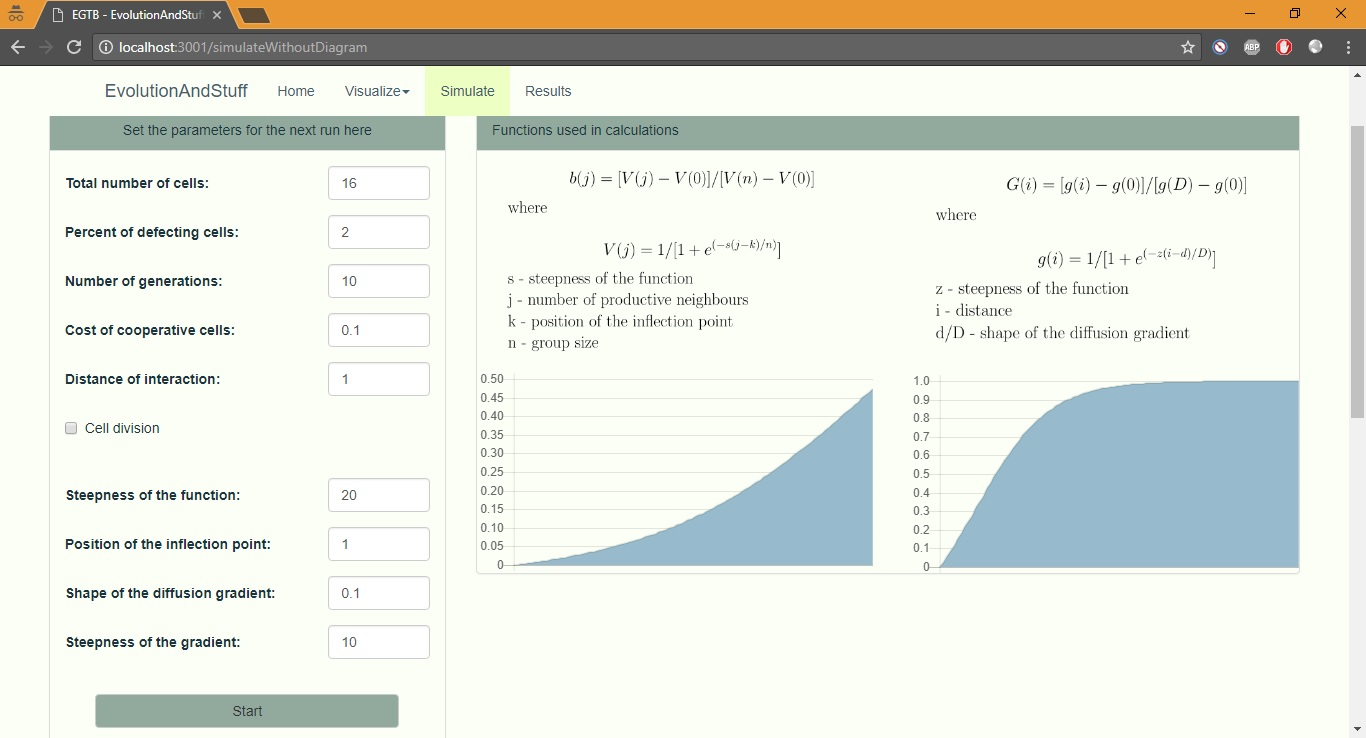
\includegraphics[width=90mm]{images/SimulationFunctionDiagrams}
	\vspace*{1mm}
	\caption{A V és g függvények alakja adott paraméterekre}
	\label{fig:SimulationFunctionDiagrams}
\end{figure}


\paragraph{Eredmények}- kezdetben már azzal is megelégedtünk, ha egy szimulációt képesek voltunk megjeleníteni, viszont egy idő után azt vettük észre, hogy milyen jó lenne ha ezeket nem kellene mindig újra és újra generálni. Így született meg az eredményeket tartalmazó rész mely megjeleníti az oldalon futtatott szimulációkat egy error bar segítségével. Mivel a bemeneti paraméterek eléggé változatosak lehetnek, így valamilyen szinten ezen adatokat a megjelenítés során szűrni kell. Ezért a felhasználó ezt köteles is megtenni mielőtt az eredményeket megtekintené, az alábbiak szerint:
\begin{itemize}
	\item defektáló sejtek aránya
	\item kooperálási költség 
	\item interakció távolsága
\end{itemize}
Ezen adatok megadása után, az összes olyan szimuláció mely kielégíti a feltételeket egyesítve lesz egy grafikonon (Ábra \ref{fig:SimulationResults}).

\begin{figure}[ht!]
	\centering
	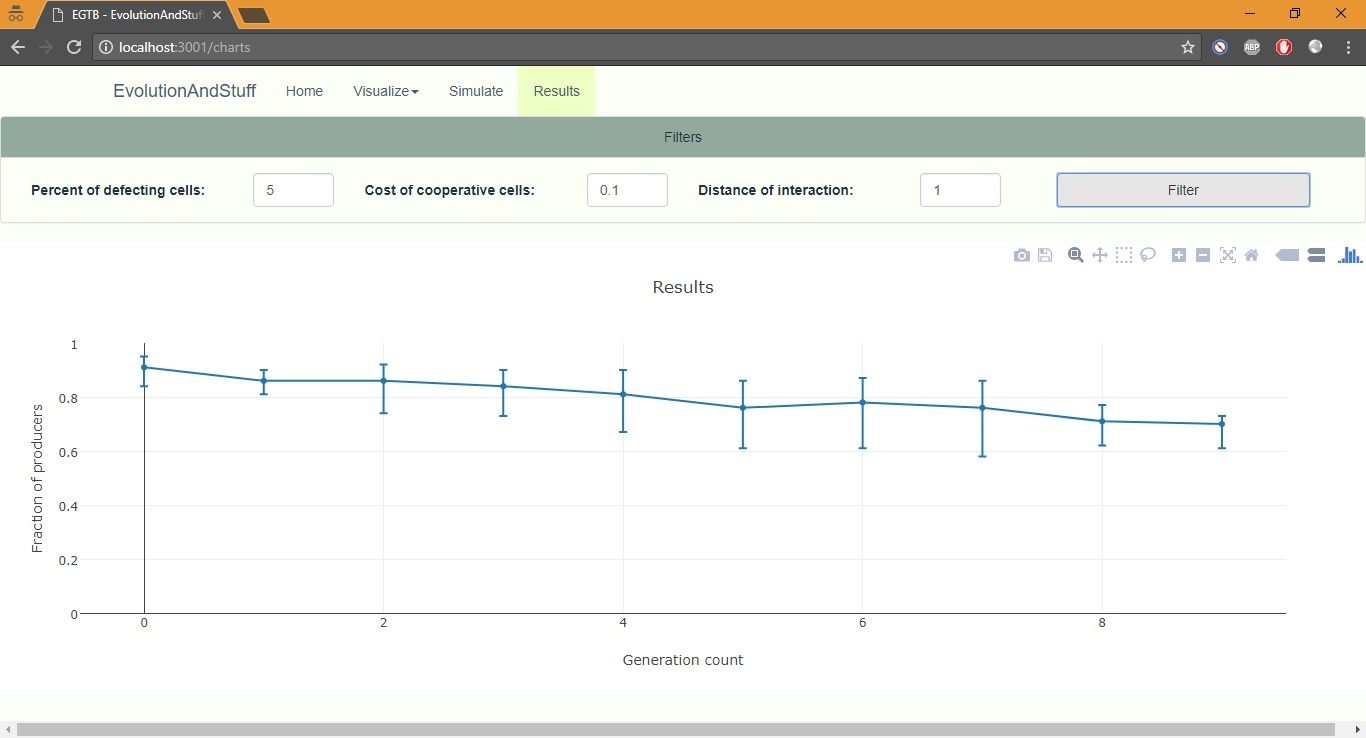
\includegraphics[width=90mm]{images/SimulationResults}
	\vspace*{1mm}
	\caption{Eddigi szimulációk eredményei}
	\label{fig:SimulationResults}
\end{figure}


\section{Felhasznált technológiák}

Annak ellenére, hogy az alkalmazás egyszerűnek tűnik egyáltalán nem az. A következőkben röviden ismertetjük a kliens oldali technológiákat (ezek részletesebben megtalálhatóak a {\color{red} Réka ref} dolgozatban), és valamivel részletesebben a szerver oldalit. Kiemeljük a folyamatos integrációt és annak megvalósításának lépéseit, valamint a tesztelési folyamatot és környezetet is ismertetjük.

\subsection{Kliens oldal}

Kliens oldalon a technológiák felhozatala eléggé változatos. Először is egy weboldal jól kell kinézzen és ezen feladatot a \textbf{Bootstrap} (\cite{soft:bootstrap}) keretrendszer tökéletesen ki is elégíti. Dinamikus oldalt lehet vele létrehozni, bármilyen eszközt együttesen lehet kezelni vele, nem csak desktopon de mobil eszközökön is jól néz ki az oldal. Kezdetben kliens oldalon nem nagyon volt bármiféle struktúra a JavaScriptben és elég hamar rá is jöttünk, hogy ez egy hatalmas probléma, a kód elég hamar átláthatatlan lett. Ezért átálltunk \textbf{AngularJS}-re (\cite{soft:angular}), mellyel már sokkal olvashatóbb kódot sikerült létrehoznunk, egyszerűbbé tette a kód bővítését is és az oldal dinamikussága is nőtt (pl. megjelentek az alertek). A Voronoi diagram megjelenítéséért a \textbf{Paper.js} (\cite{soft:paper}) a felelős, valamint itt is jelen van a Voronoi adatszerkezetet feldolgozó modul (\cite{soft:voronoiModule}). A grafikonok kirajzolására több keretrendszert is használunk. Ez azért van, mert ismertünk már egyet ami az adott feladatot kielégítette, viszont a későbbiekben új típusú diagramok jöttek be, melyekhez, mint kiderült, új keretrendszerre volt szükségünk. Így alakult, hogy a Voronoi diagram alatti grafikont a \textbf{Highcharts} (\cite{soft:highcharts}) segítségével, a V és g függvényeket (\ref{fig:SimulationFunctionDiagrams}) az AngularJS grafikonjaival, míg az error bart (\ref{fig:SimulationResults}) a \textbf{Plotly.js} (\cite{soft:plotly}) segítségével rajzoltuk ki.

\subsection{Szerver oldal}

\paragraph{NodeJS} - már a projekt kezdetekor biztosak voltunk benne, hogy egy könnyen és bárki által elérhető alkalmazásra lesz szükség, így nem volt kérdéses az, hogy webes felületet akarunk. Ezután már csak az volt a kérdéses, hogy számunkra milyen környezet lenne a legkényelmesebb, amely ha szükség van rá könnyen skálázható is. Végül a \textit{NodeJS}-re (\cite{soft:node}) esett a választásunk, hiszen ez egy egyszerű felület skálázható hálózati alkalmazások írására, valamint egy nagyon egyszerű és elterjedt nyelvet használ, a \textit{JavasSript}et. Keretrendszernek a sokak által ismert és használt \textbf{ExpressJS}-t (\cite{soft:express}) választottuk.

Tehát a szoftver egy szerverből és egy kliensből áll, melyek közötti kommunikáció a már jól megszokott HTTP-vel folyik. A fejlesztés során bizonyos szimulációs adatok JSON-beli küldözgetése túl nagy feladatnak bizonyult, így ezt más úton kellett megoldanunk. Itt megemlítenénk azt is, hogy a szerver oldalon folyik az erőforrás igényes számítások nagy része.

\paragraph{WebSocket} - olyan technológia, amely kétirányú kommunikációs csatornák kiépítését teszi lehetővé egyetlen TCP socketen keresztül. A webböngészőben futó alkalmazás képes a szerverrel való kétirányú kommunikációra (\cite{wiki:Websocket}). A már említett problémás nagyságú adatok küldözgetése ezen keresztül folyik (az [\ref{ch:appendix}] függelékben látható, hogy már 56 cella esetén is elég méretes egy üzenet. Válaszként a kliens ebből kap vissza generáció számnyit, ami 200 cella és 20 generáció esetén már elég terjedelmes üzenet).

\paragraph{Voronoi} - említettük, hogy \textit{Voronoi} diagramokkal ábrázoljuk a sejteket, így szükségünk volt egy Voronoi modulra is (\cite{soft:voronoiModule}). Ez a modul egy JavaScript implementációja Steven J. Fortune algoritmusának, mely hatékonyon dolgozik Voronoi diagramokkal, viszont csak az adatszerkezettel foglalkozik, nem képes ki is rajzolni azt.

\paragraph{MongoDB} - webalkalmazásról lévén szó szükség van egy adatbázisra is ahol a szesszió adatait el lehet tárolni, erre a \textit{MongoDB} (\cite{soft:mongodb}) jelentette a megoldást. A szimulációs eredmények lementése is ide történik, és természetesen az eredmények oldal kigenerálása során is innen vesszük ki az adatokat.

Miért pont MongoDB? Elsősorban azért, mert a Heroku platformja ingyenesen szolgáltatja számunkra és könnyű bekonfigurálni. De a legfőbb ok az, hogy az adataink JavaScript objektumokként vannak reprezentálva és a MongoDB adott számunkra egy olyan környezetet amelyben nagyon egyszerű dolgozni. Nem volt szükségünk tervezésre, hogyan nézzenek ki a relációs táblák (hisz nincs), valamint a fejlesztés során ha az objektum bármilyen szinten is változott, annak lementése ugyan olyan maradt.

\begin{figure}[ht!]
	\centering
	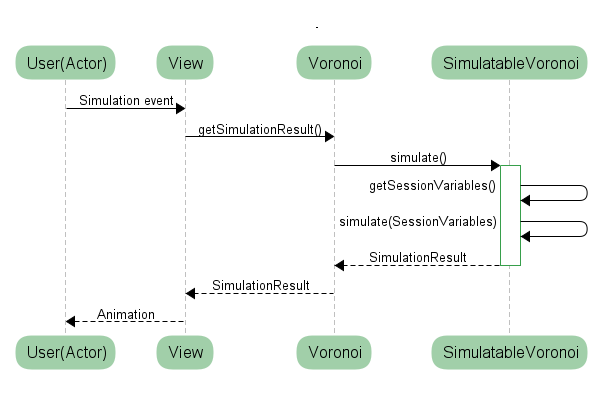
\includegraphics[width=\linewidth]{images/SimulationProcess}
	\caption{Szekvencia diagram. A szimulálási folyamat lépései}
	\label{fig:SimulationProcess}
\end{figure}

\subsection{Felhőbe vele}

Mivel az alkalmazásunk egy webalkalmazás, szükségünk volt egy szerverre, ahova ezt kitelepíthetjük. Míg régen ez egy saját szerverre telepítették mely egy statikus IP címmel rendelkezett, addig mára már sokkal könnyebb ha ezt inkább egy felhőbe rakjuk. Több ingyenesen használható felhő is létezik már, a mi választásunk a \textit{Heroku} lett (az alábbi linken érhető el az alkalmazásunk: \url{https://egtib.herokuapp.com/}).

\paragraph{Heroku} - a Heroku egy PaaS típusú felhőszolgáltató, ami annyit jelent, hogy platformot és kész szolgáltatásokat nyújt. Elég volt csak azt megmondani, hogy egy NodeJS alapú szervert akarunk üzemeltetni, ahhoz kiválasztottunk egy akármilyen adatbázist (ez lett a MongoDB), és már kész is, lehet is kitelepíteni az alkalmazást.

\subsection{Folyamatos integráció}

A folyamatos integráció egy olyan fejlesztési folyamat, ami megkönnyíti a csapatmunkában történő fejlesztést és folytonossá teszi azt. A csapat tagjai már a kezdetektől összeillesztik a kódjukat, ezek buildelése és tesztelése pedig automatikussá válik, ezzel is könnyítve a fejlesztők feladatát és gyorsabbá téve a fejlesztést.

\paragraph{TravisCI} - mivel mi sem szerettük a kitelepítést kézzel elvégezni, ezért, és persze a már fentebb is említett hasznos funkcióért is, automatizáltuk a fejlesztést a \textit{TravisCI} (\cite{soft:travis}) segítségével. A TravisCI egy folytonos integrációs platform, mely könnyen összeköthető github projektekkel, és minden egyes alkalmazás frissítéskor képes előre megadott parancsokat elvégezni (tesztelés, kitelepítés).

\paragraph{Docker} - ha az alkalmazásunkat egy \textit{Docker}-be (\cite{soft:docker}) rakjuk, akkor biztosíthatjuk azt, hogy bárhova is kerül az alkalmazásunk, mindig ugyanazon körülmények között fog futni, ez a Docker tulajdonsága.

\subsection{Tesztelés}

Semmilyen kódot nem adhatunk ki a kezünkből, ha annak minősége nincs valahogyan biztosítva. Ezt a minőséget tesztekkel lehet valamilyen szinten biztosítani, amit mi is megpróbáltunk. Köszönhetően a TravisCI-nak a tesztelés beépítése a fejlesztési folyamatba könnyen ment. Minden egyes új verzió felkerülésekor a github repositoryba, a Travis lefuttatja a teszteket és jelezi, hogy ezek között van-e olyan amely megbukott, illetve rak egy zöld pipát ha mind átment. A unit tesztjeink a \textbf{Mocha} (\cite{soft:mocha}), míg az E2E tesztjeink a \textbf{TestCafe} (\cite{soft:testcafe}) keretrendszerekben íródtak. Ezek közül kiemeljük a TestCafet, mert ez egy olyan keretrendszer melynél nincs szükség böngésző driverre, egyenesen egy előre telepített böngészőt használ, illetve fel lehet venni vele kattintásokat, azaz ki lehet vele generálni a tesztesetet és nem kell hozzá kódot írni.

\begin{figure}[ht!]
	\centering
	\includegraphics[width=\linewidth]{images/Architecture}
	\caption{A projekt architektúrája}
	\label{fig:Architecture}
\end{figure}


\chapter{A szimuláció eredményei}

Mostanra láttuk azt, hogy milyen modellekkel dolgozunk és azt is, hogy ezt szépen össze lehet gyúrni egy alkalmazásba. Azt viszont még nem láttuk, hogy ezek konkrétan milyen eredményeket is produkálnak. Az alábbiakban több szempontból is megvizsgáltuk azt, hogy a \cite{archetti2016cooperation} cikkbeli modell, illetve annak általunk kiegészített változata, hogyan viselkedik.

Kezdetben a szimuláció pontosságának megvizsgálása érdekében a már rendelkezésünkre álló bemeneti paraméterekre (melyeket Archetti is használt \cite{archetti2016cooperation}) elvégeztünk 100-100 szimulációt, minden egyes diffúziós távolságra 1-től 5-ig.

A bemeneti paraméterek a következőek voltak:
\begin{itemize}
	\item populáció mérete: 1000
	\item defektálók: 5\%
	\item generációk száma: 15
	\item kooperálók költsége: 0.01
	\item osztódás: nincs
\end{itemize}

A \eqref{eq:payoffGradient} és \eqref{eq:diffGradient} függvények paraméterei, melyeket az elkövetkezendő szimulációk során használtunk:
\begin{itemize}
	\item $s = 2$
	\item $k = 1$
	\item $d = \frac{1}{2}D$
	\item $z = 20$
\end{itemize}

Megállapítottuk, hogy ugyanarra az eredményre (Ábra \ref{fig:DistChange}) jutottunk mi is mint Archetti \cite{archetti2016cooperation}, igaz kisebb eltérések ugyan mutatkoztak. Míg mi minden esetben 100 szimulálást végeztünk, addig ő csak 10-et, így a kis eltéréseket ennek tulajdoníthatjuk.

\begin{figure}[ht!]
	\centering
	\begin{tabular}{cc}
		\includegraphics[width=0.47\linewidth]{images/dist2}
		&
		\includegraphics[width=0.47\linewidth]{images/dist4}
		\\
		\includegraphics[width=0.47\linewidth]{images/dist3}
		&
		\includegraphics[width=0.47\linewidth]{images/dist5}
		\\
	\end{tabular}
	\caption{Szimulációs eredmények a fenti paraméterekre}
	\label{fig:DistChange}
\end{figure}

Ezzel projektünk első mérföldkövét leraktuk, megbizonyosodtunk arról, hogy az általunk implementált modell visszaadja az eredetit. Most már kísérletezhetünk különböző paraméterekkel, hogy megvizsgáljuk a populáció viselkedését. Egy pár esetet a következő fejezetekben tárgyalunk.

\section{A költség és nyereség hatása}

Mint ahogyan azt már láttuk, a kooperáló sejtek termelési költsége nagyban befolyásolja a játék végkimenetelét (Ábra \ref{fig:CoopCostChange}), ami nem nagy meglepetés, hisz minél többe kerül a termelés annál jobban megéri élősködni. Az esetek többségében a defektálás a legkifizetődőbb, de alacsony költségek mellett fenntartható egy bizonyos egyensúly is a két fél között, sőt, extrém körülmények (paraméterek) mellett az is elérhető, hogy a teljes populáció a kooperálás mellett döntsön.

\begin{figure}[ht!]
	\centering
	\begin{tabular}{ccc}
		\includegraphics[width=0.32\linewidth]{images/chart001.jpeg}
		&
		\includegraphics[width=0.32\linewidth]{images/chart01.jpeg}
		&
		\includegraphics[width=0.32\linewidth]{images/chart08.jpeg}
	\end{tabular}
	\caption{A játék végkimenetele mikor a költségek rendre 0.01, 0.1 és 0.8}
\end{figure}


\section{Diffúziós távolság hatása}

Egyik legkényesebb paraméterünk amelyet változtatni lehet, az a diffúziós távolság, amely növelésével valósághűbb adatokat kaphatunk. Sajnos nem állnak rendelkezésünkre erre vonatkozó adatok a biológiából, így csak egy pár, már más által is használt értékekre végeztünk kísérleteket (Ábra \ref{fig:DiffDist}).

\begin{figure}[ht!]
	\centering
	\begin{tabular}{cc}
		\includegraphics[width=0.47\linewidth]{images/diffdist2}
		&
		\includegraphics[width=0.47\linewidth]{images/diffdist5}
	\end{tabular}
	\caption{A játék végkimenetele két diffúziós távolságra. A paraméterek: 160 sejt, 5\% defektáló, 0.3 költség, távolság: 2 illetve 5}
	\label{fig:DiffDist}
\end{figure}

Megfigyelhető, hogy a távolság növekedésével a defektáló sejtek jóval könnyebben terjednek el, nem csak a közvetlen szomszédokat befolyásolják, hanem a tőlük távolabb elhelyezkedőeket is. Meg kell jegyeznünk, hogy ezt a paramétert a hasnyálmirigyrák esetén megállapították \cite{archetti2015heterogeneity}, valamint az is biztos, hogy az esetek túlnyomó részében ez az érték 5-10-től 30-60-ig terjedhet \cite{archetti2016cooperation}.
%További megvalósítandó feladataink közé tartozik egy olyan funkció mely révén ellenanyagot juttathatunk a daganatba, vagy egy terápiát alkalmazhatunk.
\section{Osztódásra képes populációk}

Eddigi szimulációink során a populáció mérete állandó volt, és egy adott modellt követett. A már említett Gompertz-modellt (\ref{eq:gompertz}) beépítve a modellbe és az alkalmazásba (a felhasználói webes felületen csak egy checkbox, azaz akar-e a felhasználó osztódást) újabb szimulációkat futtattunk. Az \ref{fig:Divide} ábra szemlélteti azt az esetet amikor a sejtek osztódni is képesek és nem csak stratégiát váltani. 

\begin{figure}[ht!]
	\centering
	\begin{tabular}{cc}
		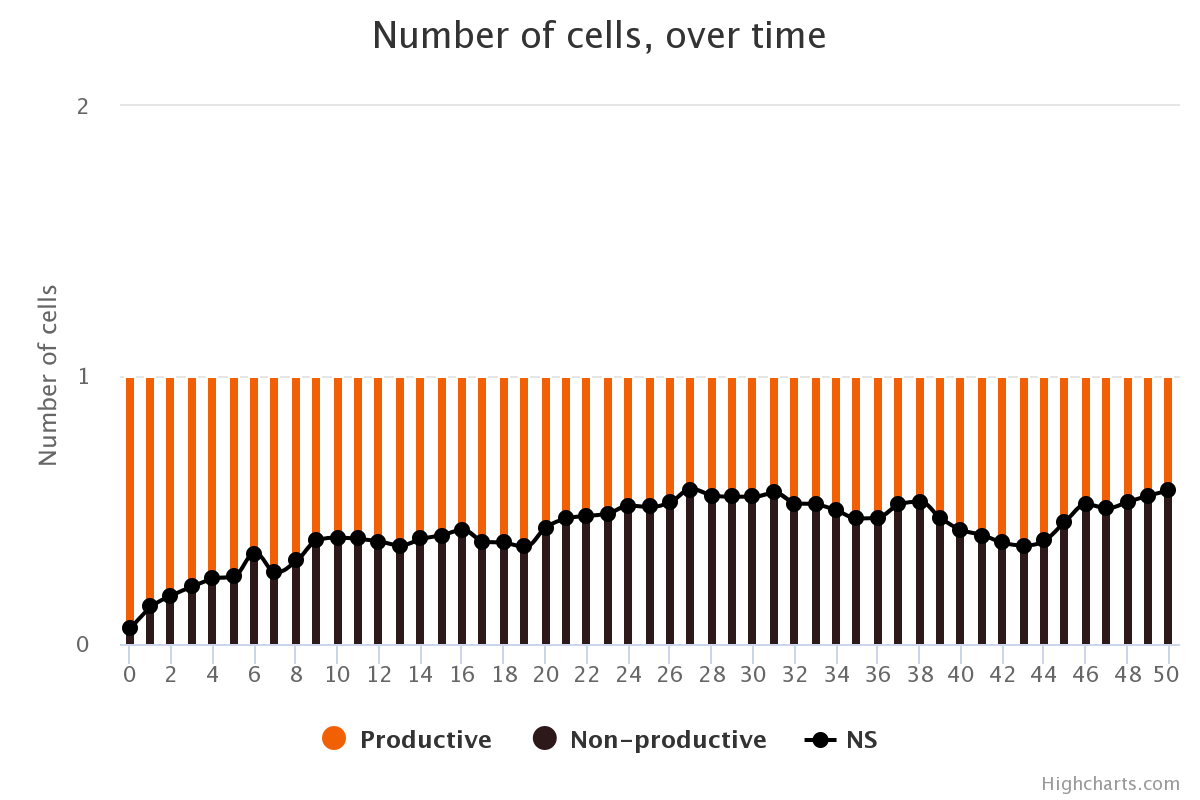
\includegraphics[width=0.47\linewidth]{images/nemosztodik}
		&
		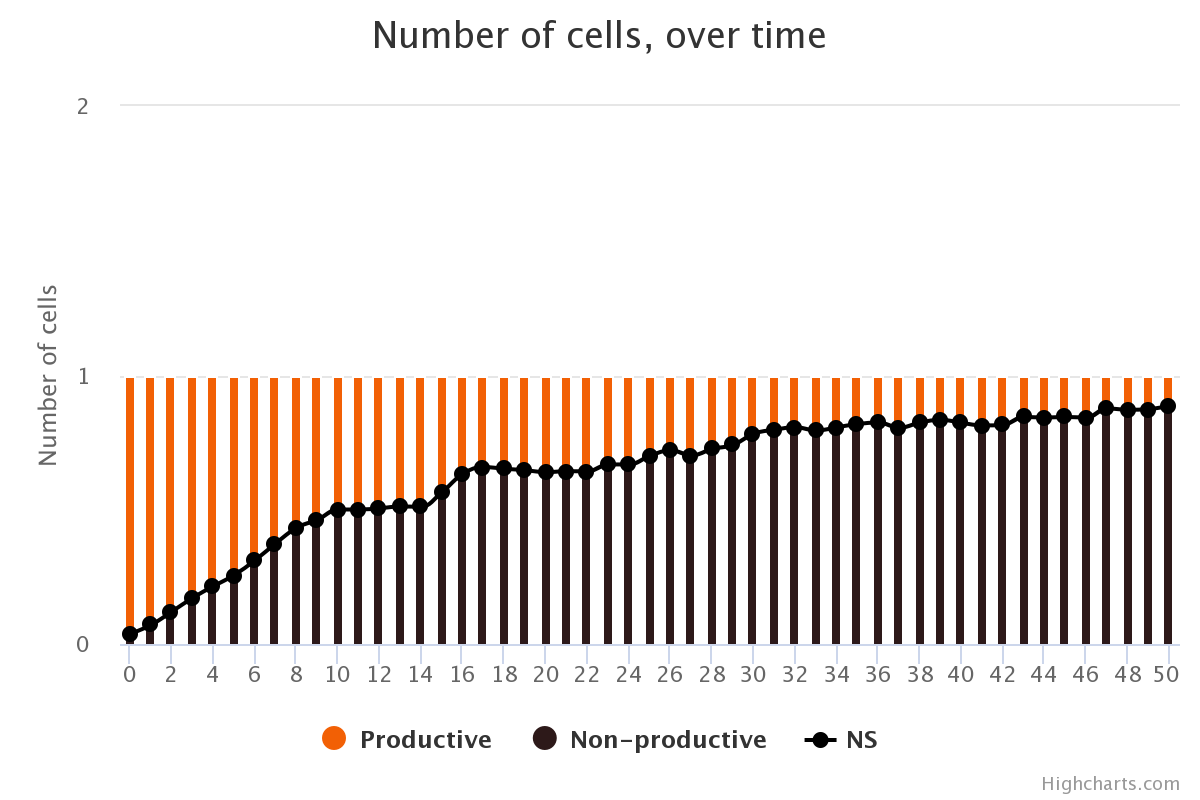
\includegraphics[width=0.47\linewidth]{images/osztodik}
	\end{tabular}
	\caption{Az első esetben a sejtek nem osztódtak míg a másodikban igen}
	\label{fig:Divide}
\end{figure}

Igaz, hogy a stratégia váltást fel lehet fogni úgy mint egy fajta osztódást, ahol az a sejt amelyik átveszi a stratégiát meghal és annak a sejtnek a másolata jön létre ugyanazon a területen akitől azt átveszi, de a valóságban a defektáló sejtek nem csak területileg terjednek el, hanem számosságban is túlnövik a kooperálókat.
Az osztódás során létrejött új sejtek képesek felgyorsítani a defektálók terjedését, de ezen területen még további kísérletek szükségesek, hogy pontosabb képet kapjunk arról, hogy ez mennyire befolyásolja a játék végkimenetelét.

Felhasználva a fenti paramétereket legeneráltunk egy újabb populációt mely már osztódásra képes (\ref{table:osztodik} táblázat), és ezen eredményeket összevetettük azon modellel ahol nem volt osztódás (\ref{table:nemOsztodik} táblázat). Látható, hogy a kooperálók aránya (CoopPerc) kisebb amikor a sejtek osztódnak, de a szórása is nő.

\begin{table}[htb]
	\centering
	\caption{Osztódás nélküli modell \label{table:nemOsztodik}}
	\begin{tabular}{ | l | l | l | l | l | l | l | l | l | l | l | l | }
		\hline
		\multirow{3}{*}{D = 2}
		& Generáció & 1 & 2 & 3 & 4 & 5 & 6 & 7 & 8 & 9 & 10 \\ \cline{2-12}
		& CoopPerc & 0.91 & 0.91 & 0.85 & 0.81 & 0.77 & 0.75 & 0.73 & 0.71 & 0.69 & 0.68 \\ \cline{2-12}
		& stdev & 0.01 & 0.01 & 0.02 & 0.03 & 0.03 & 0.03 & 0.05 & 0.05 & 0.05 & 0.06 \\ \hline
		\multirow{3}{*}{D = 3}
		& Generáció & 1 & 2 & 3 & 4 & 5 & 6 & 7 & 8 & 9 & 10 \\ \cline{2-12}
		& CoopPerc & 0.9 & 0.9 & 0.83 & 0.77 & 0.72 & 0.68 & 0.66 & 0.64 & 0.62 & 0.6 \\ \cline{2-12}
		& stdev & 0.02 & 0.02 & 0.03 & 0.04 & 0.04 & 0.05 & 0.04 & 0.05 & 0.05 & 0.04 \\ \hline
	\end{tabular}
\end{table}

\begin{table}[htb]
	\centering
	\caption{Osztódást használó modell}
	\label{table:osztodik}
	\begin{tabular}{ | l | l | l | l | l | l | l | l | l | l | l | l | }
		\hline
		\multirow{3}{*}{D = 2}
		& Generáció & 1 & 2 & 3 & 4 & 5 & 6 & 7 & 8 & 9 & 10 \\ \cline{2-12}
		& CoopPerc & 0.87 & 0.87 & 0.79 & 0.74 & 0.7 & 0.67 & 0.64 & 0.61 & 0.59 & 0.57 \\ \cline{2-12}
		& stdev & 0.02 & 0.02 & 0.03 & 0.04 & 0.05 & 0.06 & 0.07 & 0.05 & 0.07 & 0.07 \\ \hline
		\multirow{3}{*}{D = 3}
		& Generáció & 1 & 2 & 3 & 4 & 5 & 6 & 7 & 8 & 9 & 10 \\ \cline{2-12}
		& CoopPerc & 0.89 & 0.9 & 0.82 & 0.75 & 0.7 & 0.66 & 0.62 & 0.59 & 0.56 & 0.54 \\ \cline{2-12}
		& stdev & 0.03 & 0.04 & 0.05 & 0.06 & 0.08 & 0.08 & 0.08 & 0.09 & 0.09 & 0.09 \\ \hline
	\end{tabular}
\end{table}

\chapter{Összegzés}

Dolgozatunkban sikerült az \cite{archetti2016cooperation} cikkben felállított modellt egy új, dinamikus jelleggel, a sejtosztódással kiterjeszteni. Megtudtuk hogyan befolyásolják egyes paraméterek a játék végkimenetelét, valamint a két modell alapján kapott eredmények összehasonlításával megvizsgáltuk, hogyan változik a populációk összetétele ha az osztódást is figyelembe vesszük.

Elmondhatjuk, hogy sikerült egy olyan szoftvert létrehoznunk mely segítségével jobban megérhetjük, hogy mi is történik egy daganaton belül. Fő erőssége a kísérletezésben rejlik, de kutatási vagy akár tanítási célokra is fel lehet használni. Webes alkalmazás révén egyszerűen elérhető, bárki által használható. Letisztult felülete átláthatóvá és könnyen használhatóvá teszi. Tudtunk szerint, a játékelmélet ezen területén, ez az első önálló szoftver, amely 
\begin{itemize}
	\item interaktívan mutatja be a sejtpopulációk változását
	\item ezen bemutatáshoz voronoi diagramot használ
	\item nem igényel programozási tudást, hiszen képes szimulációkat végezni pár kattintással
\end{itemize}

Természetesen hiányosságai is vannak, melyeket a jövőben szeretnénk pótolni. Rendkívül hasznos lenne azon funkció mely során egy terápiát (pl. kemoterápia) alkalmazunk, vagy ellenanyagokat juttatunk be, melyek a termelést, annak költségét befolyásolják. Komoly kihívásnak számít az, hogy különböző ráktípusokra meghatározzuk az őket leíró paramétereket. A számítások hatékonyságágának növelése is egy fontos feladat, ami maga után vonná azt a tényt, hogy nagyobb populációkkal és diffúziós gradienssel is szimulálhatnánk. 
Jelenleg csak papíron létezik több fajta stratégia \cite{hummert2014evolutionary} de a közeljövőben be szeretnénk vezetni még legalább egyet mint válaszható opciót.

Az általunk végzett szimulációk arra engednek következtetni, hogy a sejtek játéka bizonyos határokon belül leírja a daganatok viselkedését és hisszük azt, hogy a játékelmélettel ezen területet ki lehet aknázni.


{ \renewcommand{\baselinestretch}{0.8}\normalsize %
  \setlength{\itemsep}{-2.4mm}
  \setlength{\bibspacing}{0.67\baselineskip}
  \bibliographystyle{abbrvnat_hu}
  \bibliography{articles}
}

\end{document}
